\documentclass{standalone}
%
\usepackage{tikz}
\usetikzlibrary{backgrounds,shapes.callouts}
\usepackage{tkz-euclide}
\usepackage{xcolor}
\usepackage{ifthen}
%
\definecolor{space}{HTML}{1F2C4E}
\definecolor{earth}{HTML}{0089FA}
\definecolor{dida}{HTML}{FFDE00}
\definecolor{title}{HTML}{FBA706}
\definecolor{moon}{HTML}{AFAFAF}
%
\usepackage{fontspec}
\setmainfont{Open Dyslexic}
%
\title{La leggenda del tombino nello spazio}
\begin{document}
	\tikzset{
		partial ellipse/.style args = {#1:#2:#3}{insert path={+ (#1:#3) arc (#1:#2:#3)}},
		notice/.style  = { draw, ellipse callout, callout relative pointer={#1} },
	}
	\begin{tikzpicture}[background rectangle/.style={fill=white},show background rectangle,>={[inset=0,angle'=27]Stealth}]
		%title
		\draw [black,ultra thick] (1,1) rectangle (29,-1);
		\node at (15,0) {\textcolor{black}{\fontsize{35}{36}\selectfont La leggenda del tombino nello spazio}};
		%
		\begin{scope}[shift={(0,-5)}]
			\node at (15,0) {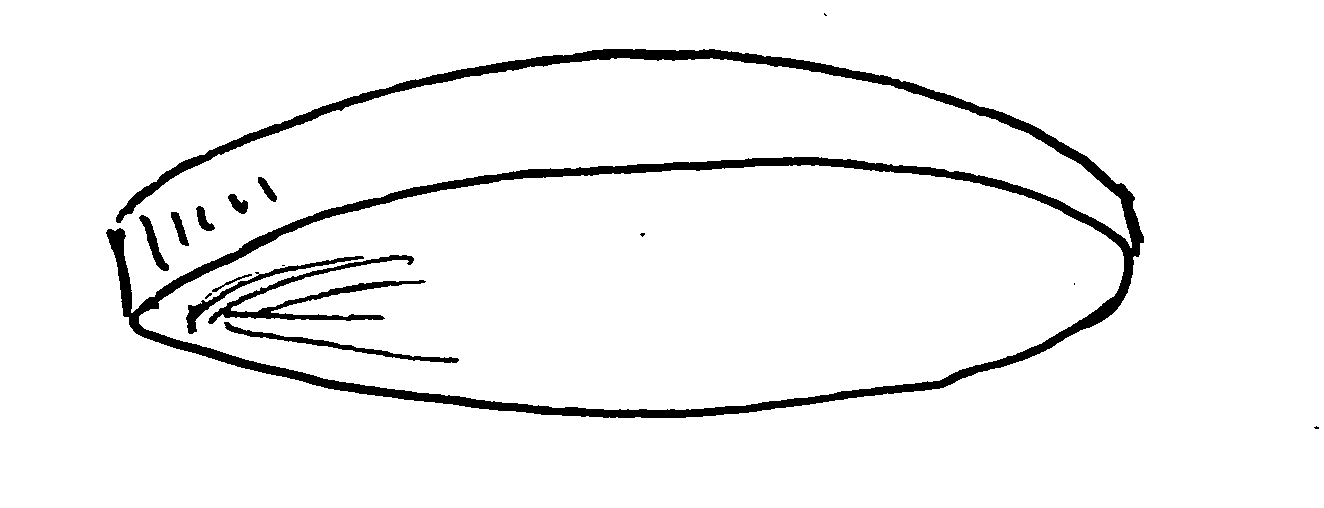
\includegraphics[width=10cm]{img-tombino/tombino01}};
			\node (example-textwidth-2) [notice={(-1,-0.5)}, ultra thick, right, align=center, text width=6cm, color=black, fill=white, font=\fontsize{23pt}{24pt}\selectfont] at (5,-4) {Guarda, mamma! un UFO!};
			\node (example-textwidth-2) [notice={(1,0.5)}, ultra thick, right, align=center, text width=6cm, color=black, fill=white, font=\fontsize{23pt}{24pt}\selectfont] at (15,-4) {Aspetta che avviso la C.A.S.A.};
			\node (example-textwidth-2) [right, align=left, text width=11cm, color=black, font=\fontsize{18pt}{19pt}\selectfont] at (15,-7) {C.A.S.A.: Cosmica Agenzia Spaziale Alienata};
		\end{scope}
		%
		\begin{scope}[shift={(0,-16)}]
			\node at (15,0) {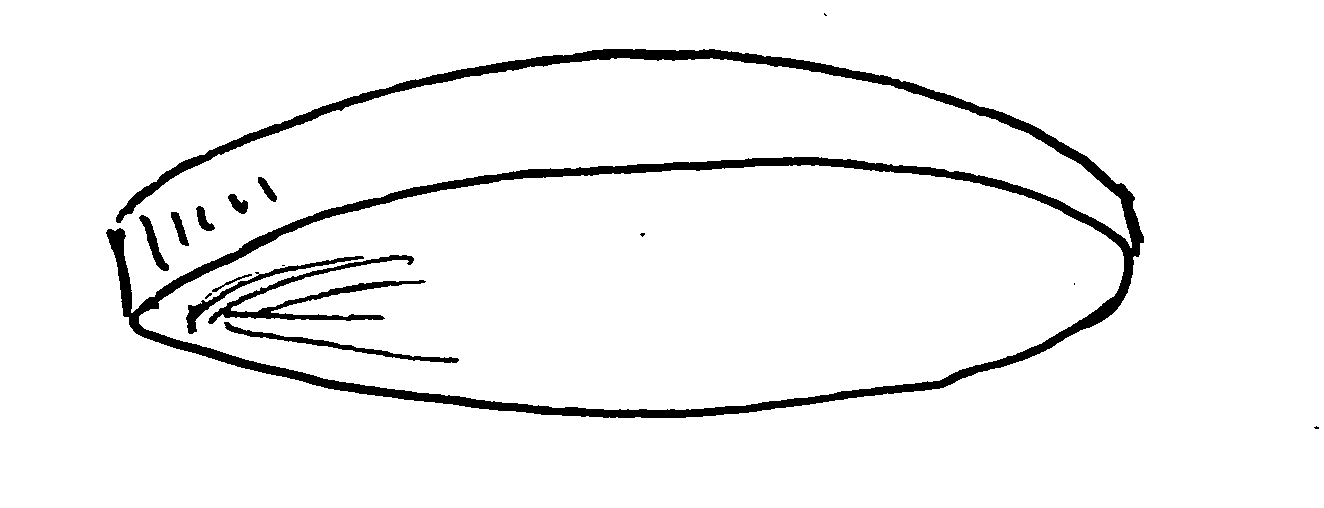
\includegraphics[width=10cm]{img-tombino/tombino01}};
			\node (example-textwidth-2) [notice={(-1,-0.5)}, ultra thick, right, align=center, text width=6cm, color=black, fill=white, font=\fontsize{23pt}{24pt}\selectfont] at (5,-4) {Una signora ci ha segnalato un UFO...};
			\node (example-textwidth-2) [notice={(1,0.5)}, ultra thick, right, align=center, text width=6cm, color=black, fill=white, font=\fontsize{23pt}{24pt}\selectfont] at (15,-4) {Controllo al volo col satellite!};
		\end{scope}
		%
		\begin{scope}[shift={(0,-26)}]
			\node at (15,0) {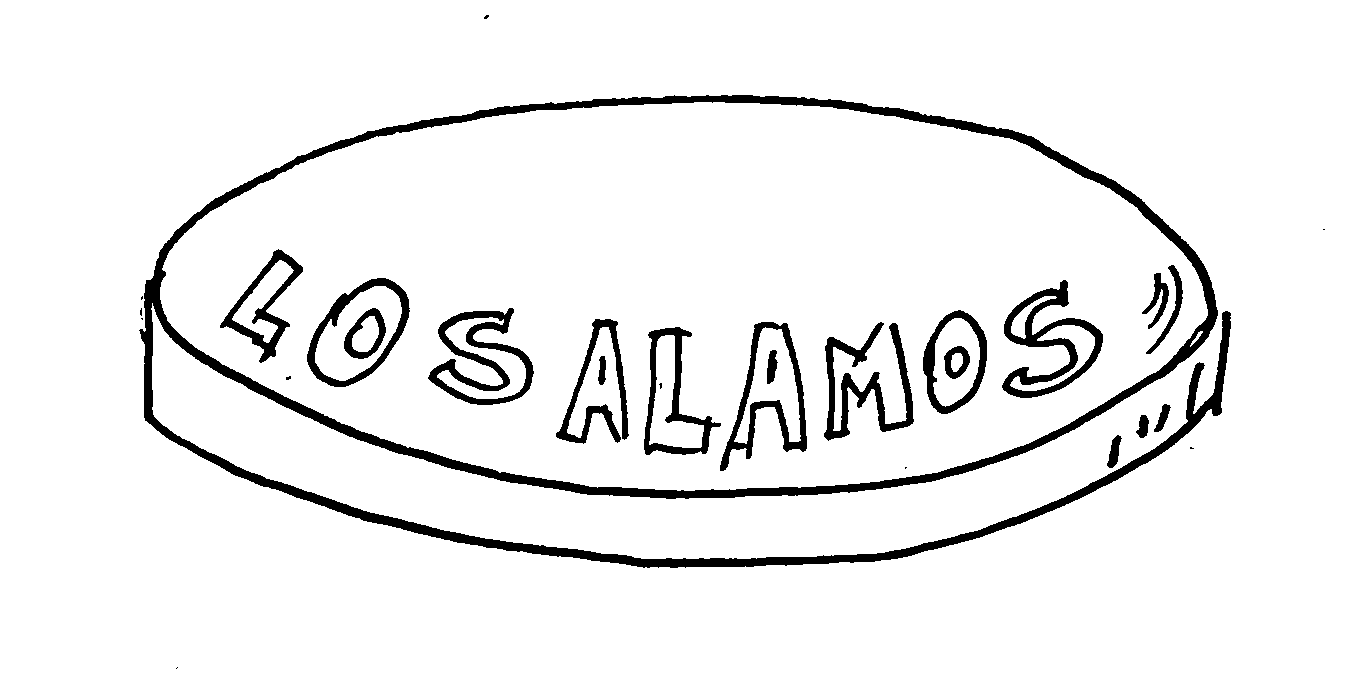
\includegraphics[width=10cm]{img-tombino/tombino02}};
			\node (example-textwidth-2) [notice={(-1,-0.5)}, ultra thick, right, align=center, text width=2cm, color=black, fill=white, font=\fontsize{23pt}{24pt}\selectfont] at (5,-4) {...};
			\node (example-textwidth-2) [notice={(1,0.5)}, ultra thick, right, align=center, text width=6cm, color=black, fill=white, font=\fontsize{23pt}{24pt}\selectfont] at (15,-4) {Ah no! E' solo un tombino!};
		\end{scope}
		%
		\begin{scope}[shift={(0,-35)}]
			\draw[color=black,fill=white,ultra thick] (1,2) rectangle (29,-2);
			\node at (3,0) {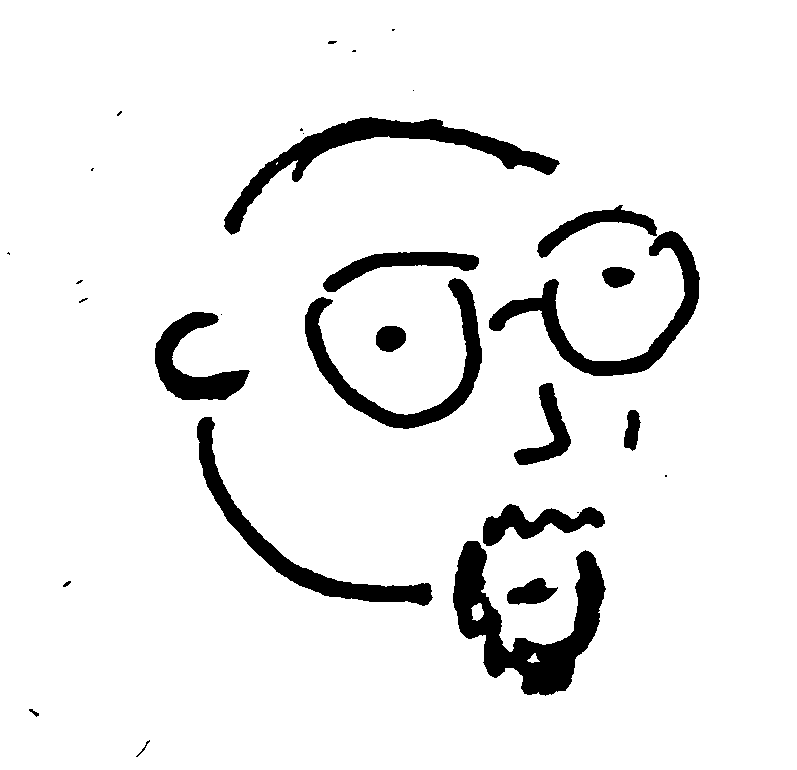
\includegraphics[width=5cm]{img-tombino/io_sx}};
			\node (example-textwidth-2) [right, align=left, text width=22cm, color=black, font=\fontsize{21pt}{22pt}\selectfont] at (6,0) {In effetti, ad agosto del 1957, durante il test nucleare Pascal-B condotto sottoterra, un tombino posto alla fine di uno sfiatatoio lungo 150 m venne lanciato in aria. Forse nello spazio.};
		\end{scope}
		%
		\begin{scope}[shift={(0,-50)}]
			\node at (15,0) {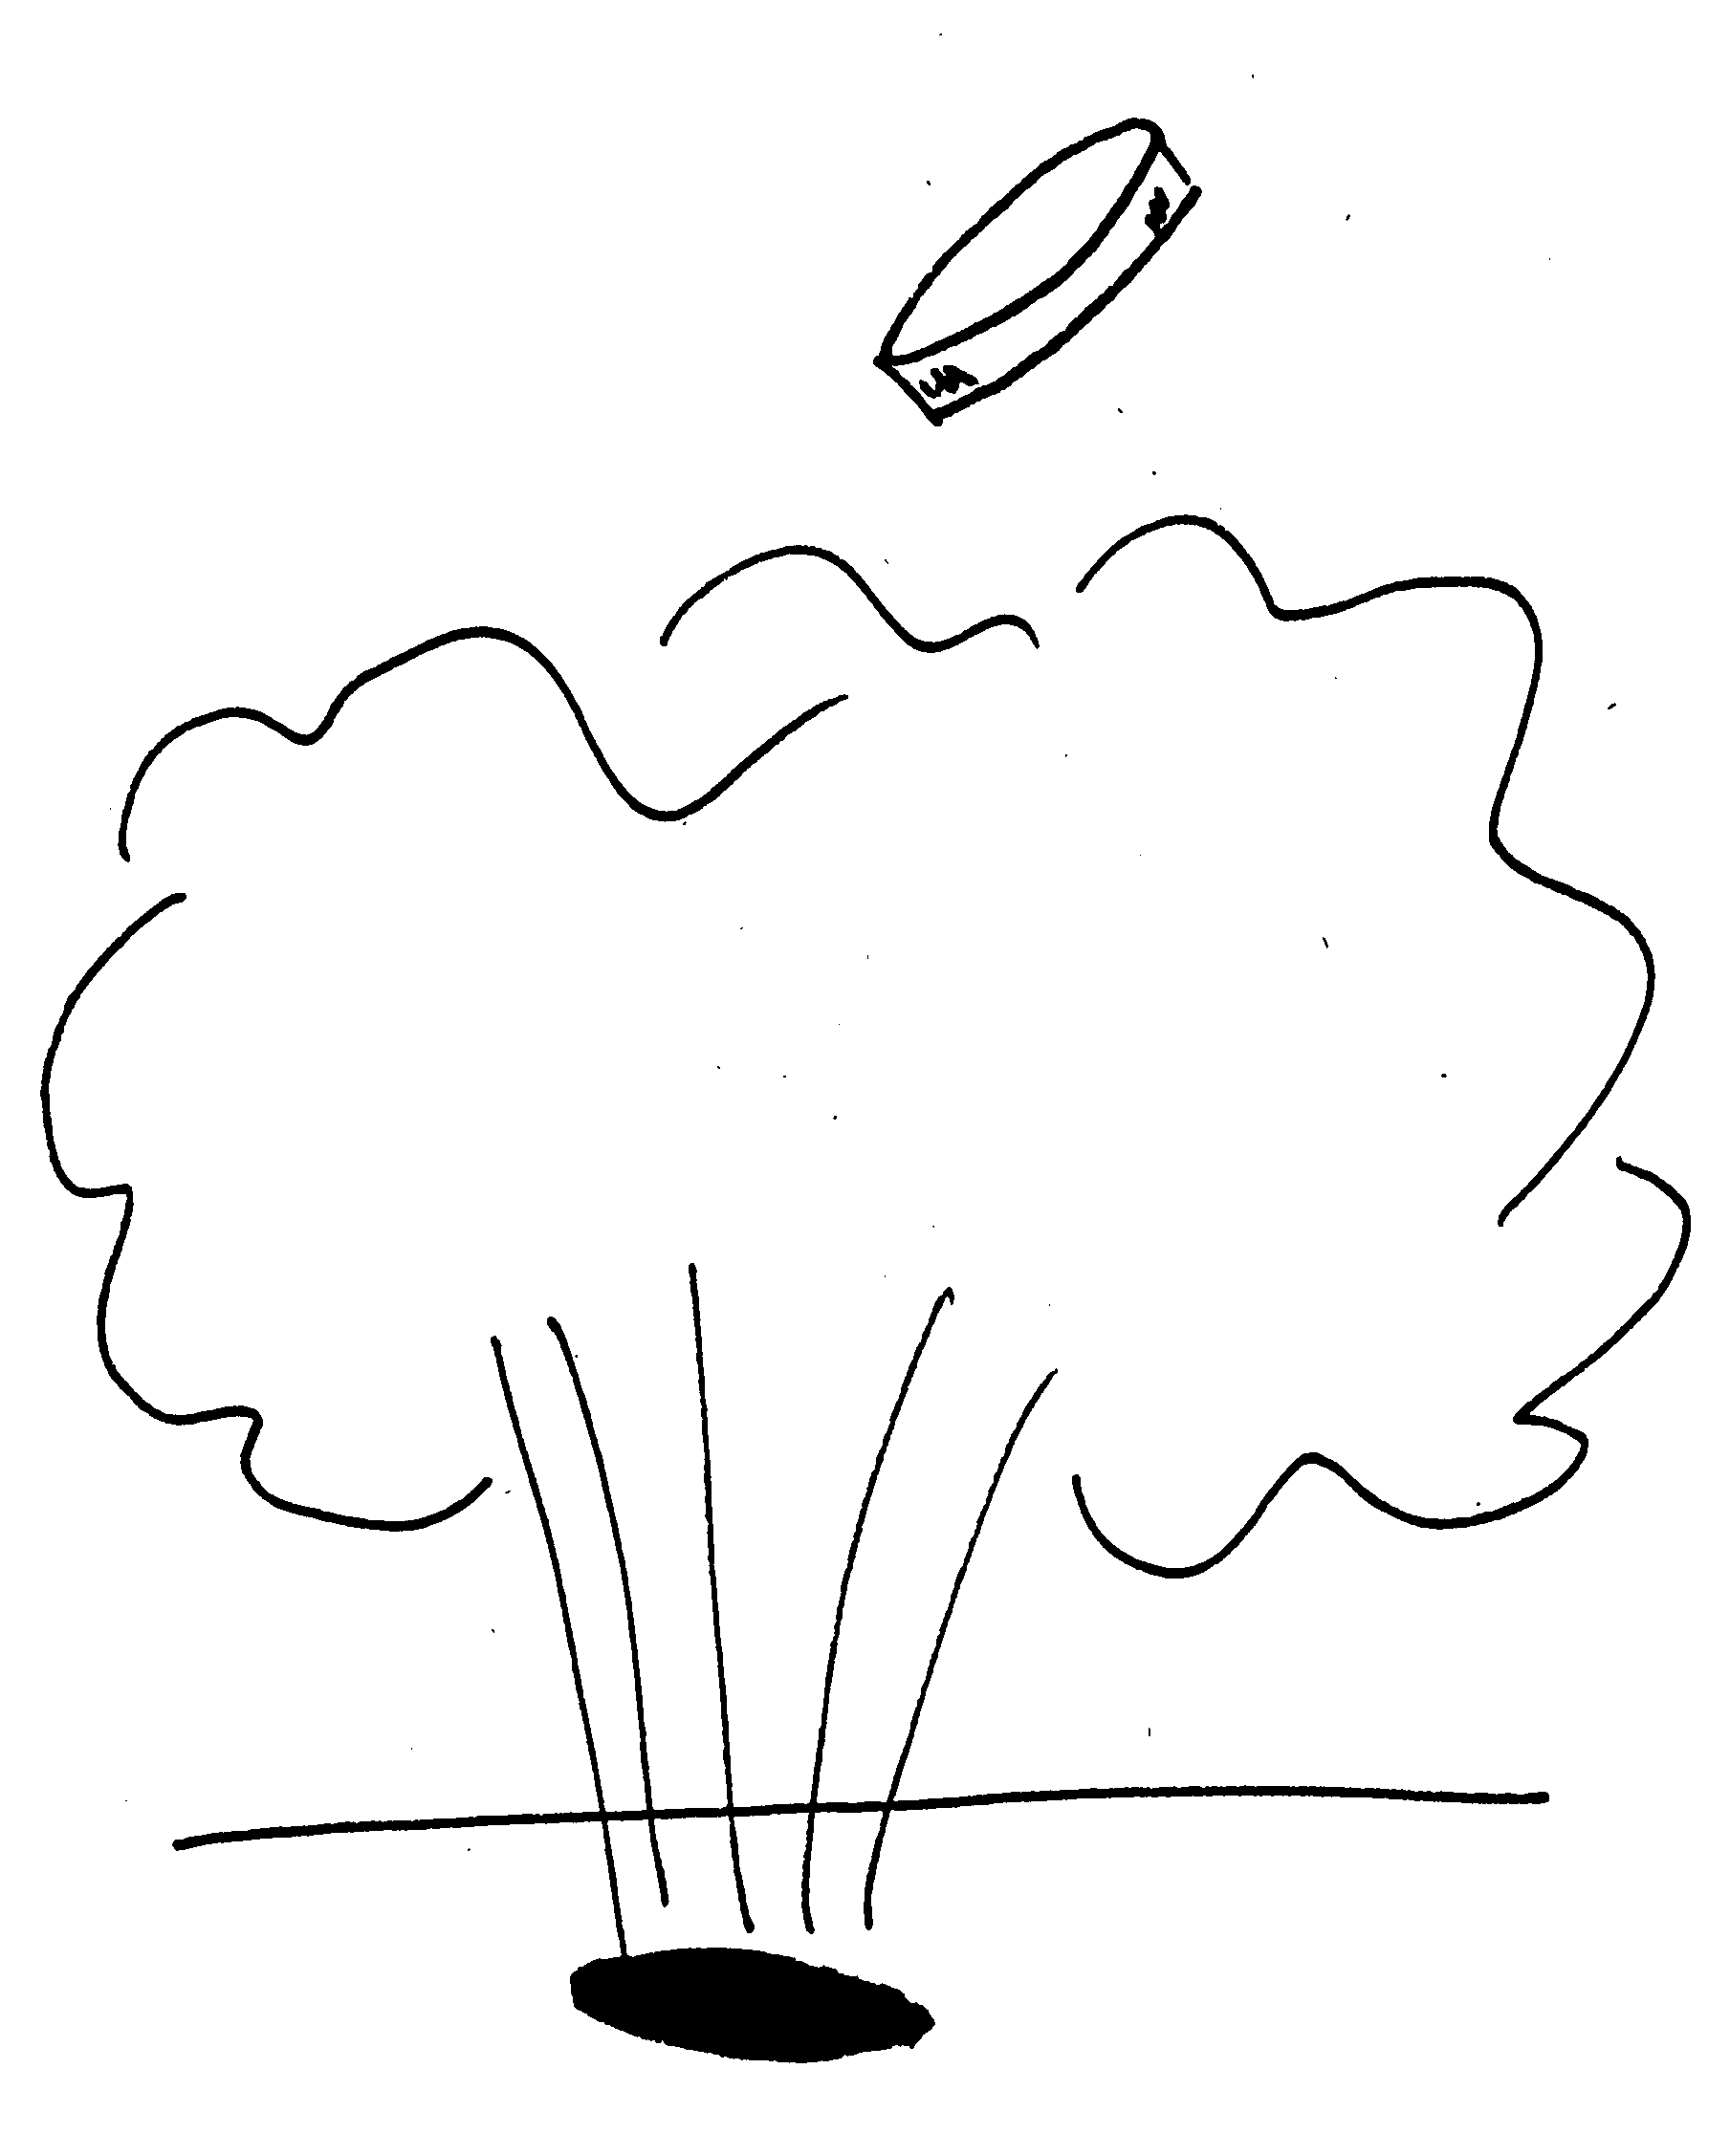
\includegraphics[width=20cm]{img-tombino/esplosione}};
		\end{scope}
		%
		\begin{scope}[shift={(0,-65)}]
			\draw[color=black,fill=white,ultra thick] (1,2) rectangle (29,-2);
			\node at (3,0) {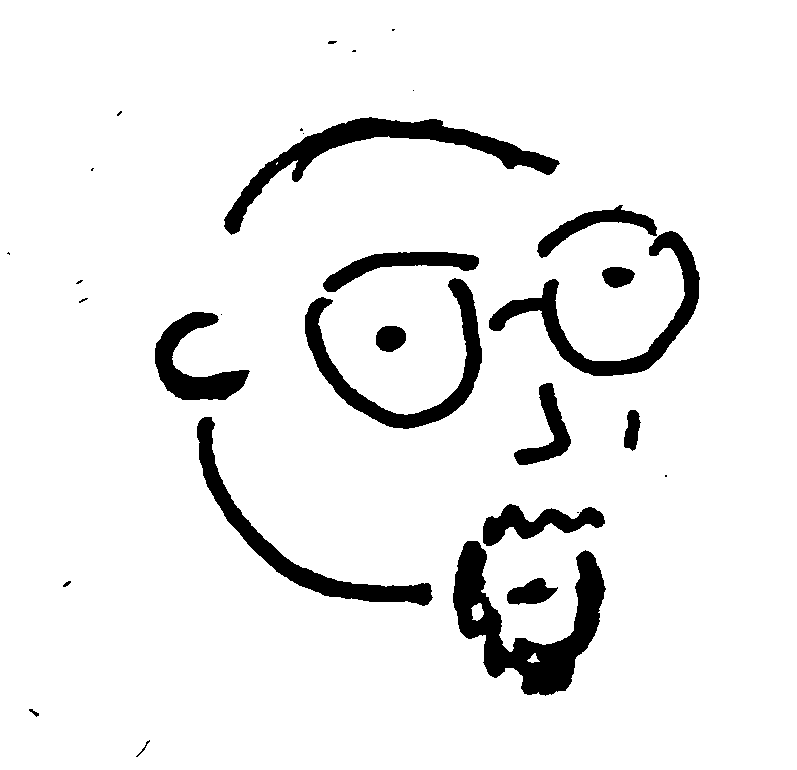
\includegraphics[width=5cm]{img-tombino/io_sx}};
			\node (example-textwidth-2) [right, align=left, text width=22cm, color=black, font=\fontsize{21pt}{22pt}\selectfont] at (6,0) {Dopo una serie di stressanti insistenze da parte del supervisore \textbf{Bill Ogle} (a sinistra), \textbf{Robert Brownlee} (a destra) disse che il tombino sarebbe potuto anche finire nello spazio};
		\end{scope}
		%
		\begin{scope}[shift={(0,-73)}]
			\node at (7,0) {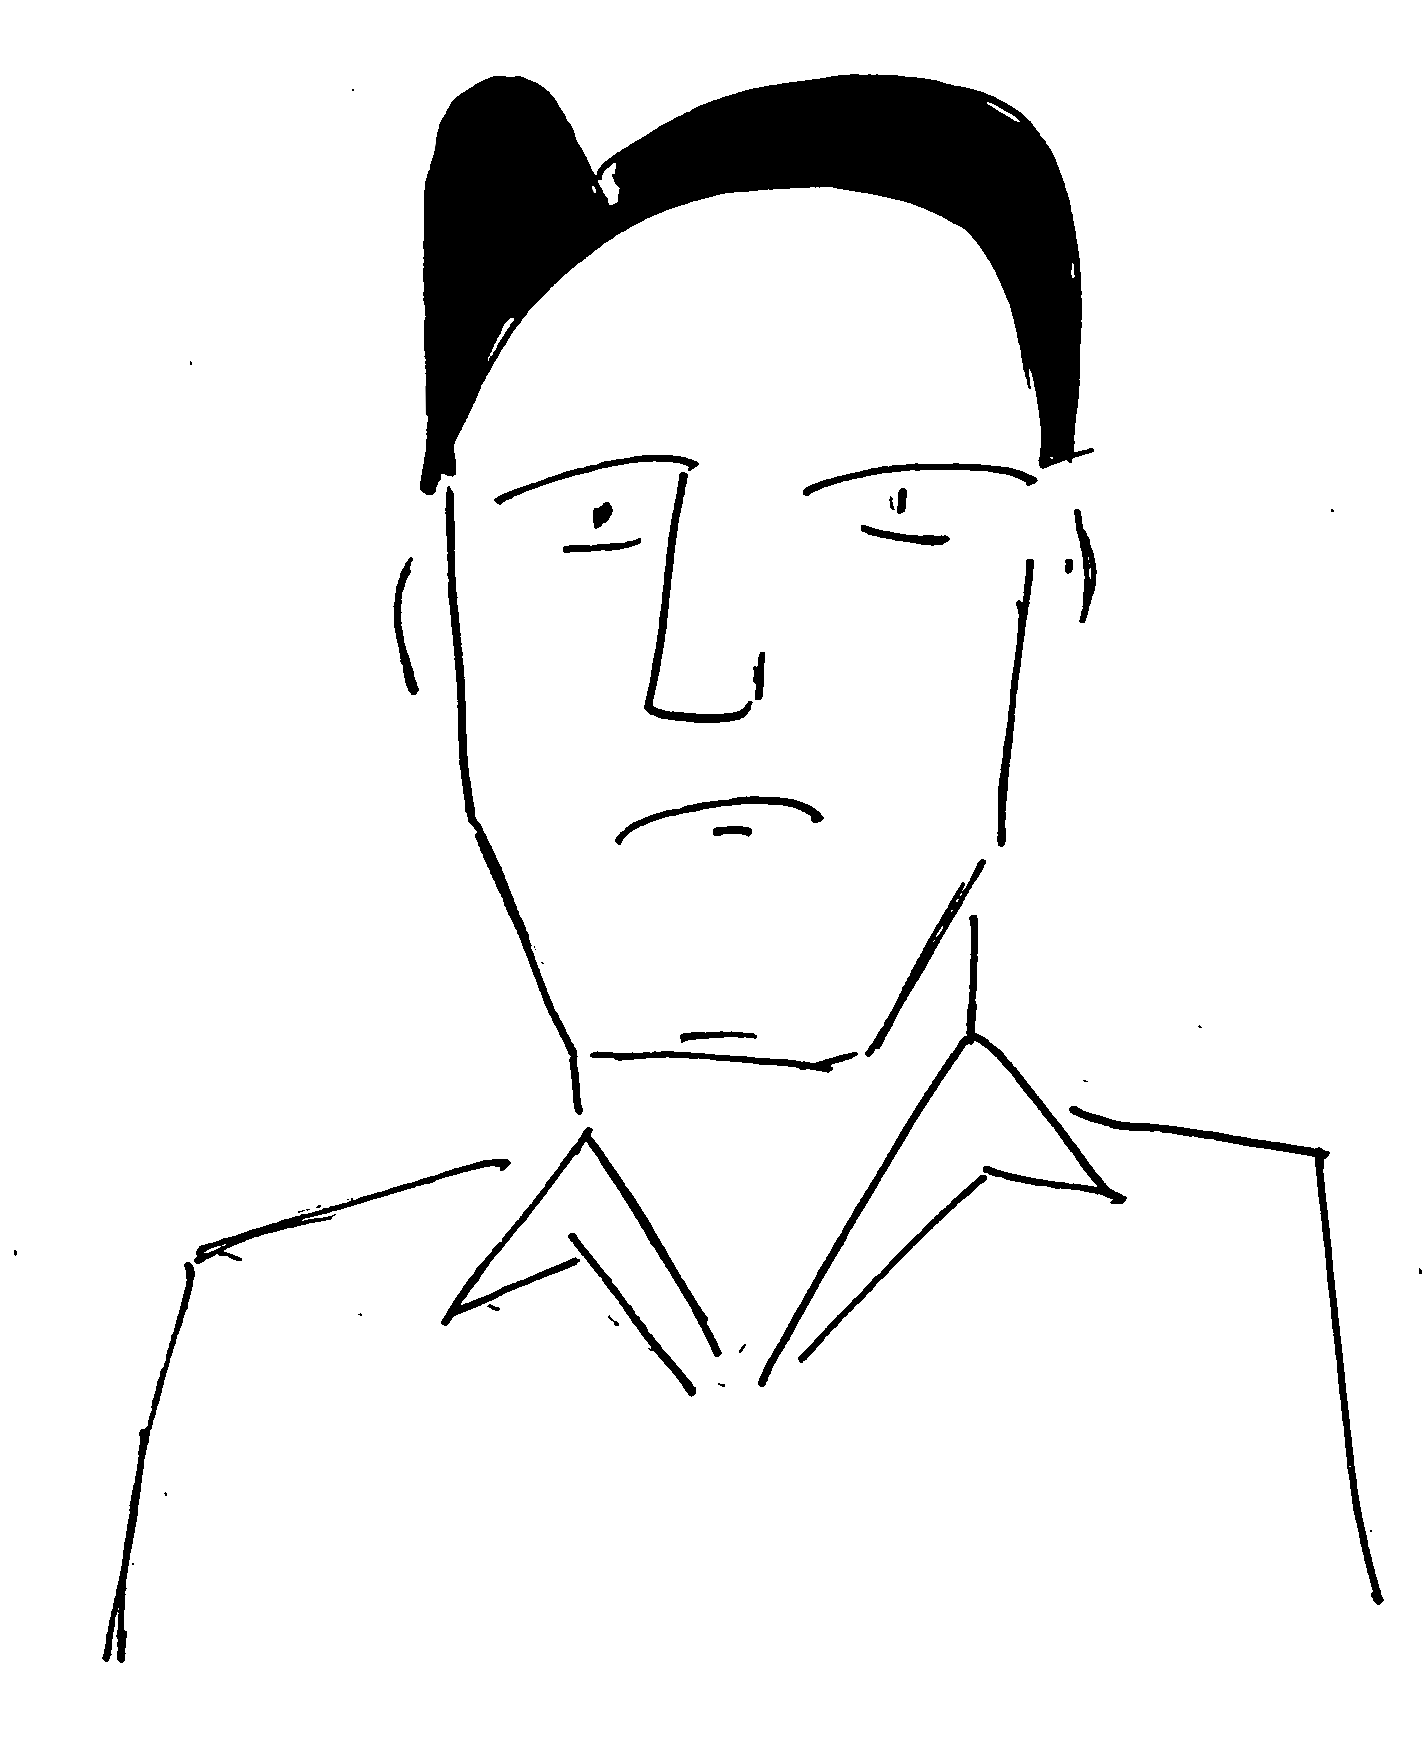
\includegraphics[width=8cm]{img-tombino/bill_ogle}};
			\node at (21,0) {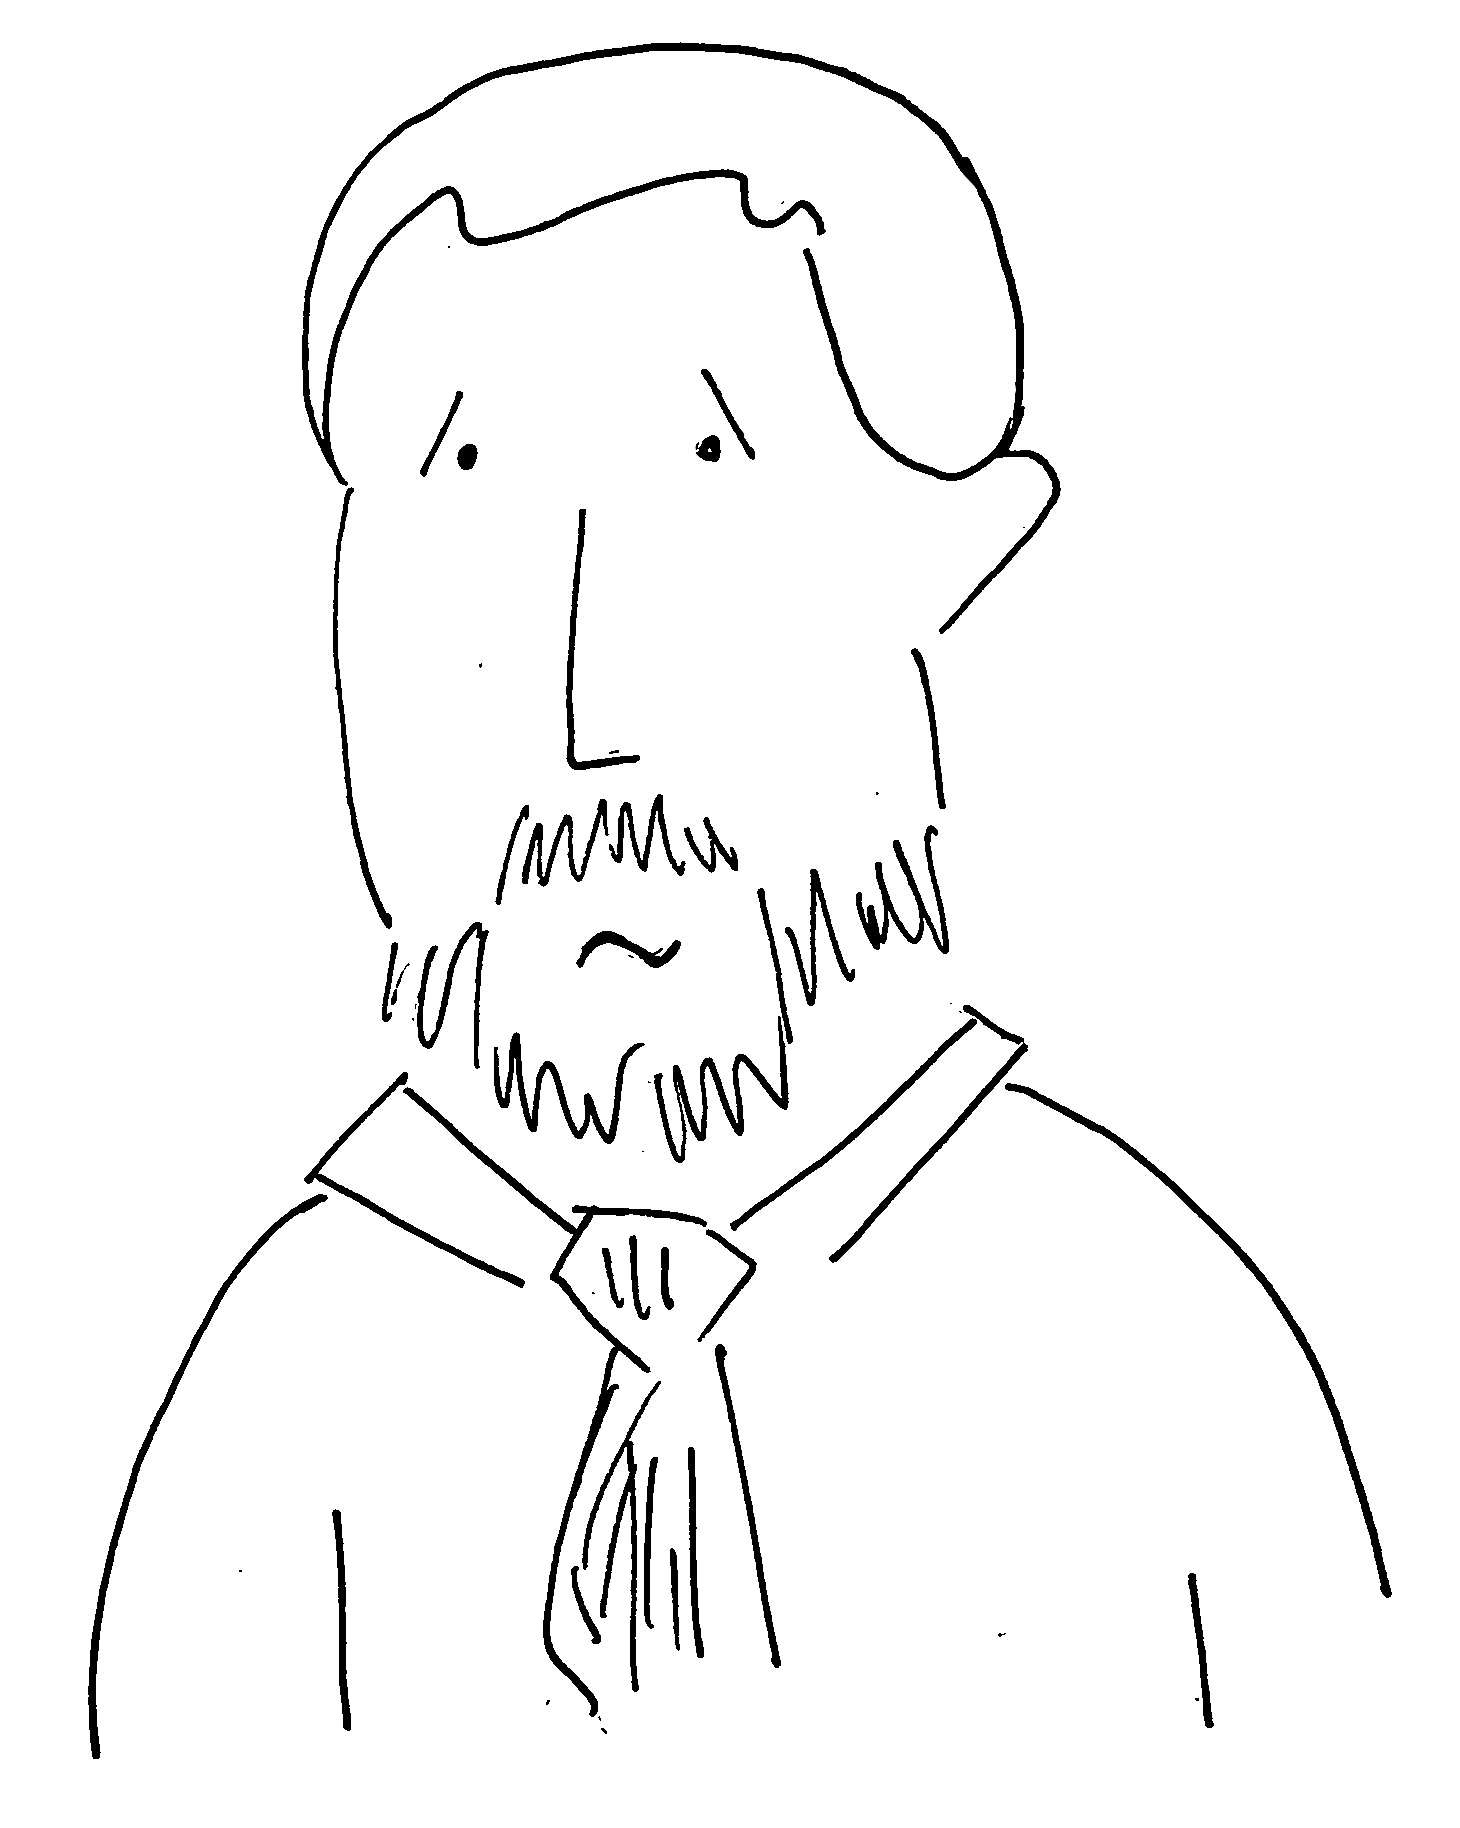
\includegraphics[width=8cm]{img-tombino/robert_brownlee}};
		\end{scope}
		%
		\begin{scope}[shift={(0,-77)}]
			\node (example-textwidth-2) [notice={(-1,-0.5)}, ultra thick, right, align=center, text width=6cm, color=black, fill=white, font=\fontsize{23pt}{24pt}\selectfont] at (5,-4) {Quanto tempo impiegherebbe l'onda d'urto ad arrivare in cima?};
			\node (example-textwidth-2) [notice={(1,-0.5)}, ultra thick, right, align=center, text width=6cm, color=black, fill=white, font=\fontsize{23pt}{24pt}\selectfont] at (15,-4) {Circa 31 millisecondi...};
			%
			\node (example-textwidth-2) [notice={(-1,-0.5)}, ultra thick, right, align=center, text width=6cm, color=black, fill=white, font=\fontsize{23pt}{24pt}\selectfont] at (5,-12) {E cosa potrebbe succedere?};
			\node (example-textwidth-2) [notice={(1,-0.5)}, ultra thick, right, align=center, text width=7cm, color=black, fill=white, font=\fontsize{23pt}{24pt}\selectfont] at (15,-12) {La pressione e la temperatura sono tali che il tombino, per quanto saldato, salterebbe via...};
			%
			\node (example-textwidth-2) [notice={(-1,-0.5)}, ultra thick, right, align=center, text width=6cm, color=black, fill=white, font=\fontsize{23pt}{24pt}\selectfont] at (5,-20) {E quanto va veloce?};
			\node (example-textwidth-2) [notice={(1,-0.5)}, ultra thick, right, align=center, text width=7cm, color=black, fill=white, font=\fontsize{23pt}{24pt}\selectfont] at (15,-20) {I miei calcoli su questo punto sono irrilevanti. Valgono solo relativamente all'onda d'urto...};
			%
			\node (example-textwidth-2) [right, align=left, text width=22cm, color=black, font=\fontsize{23pt}{24pt}\selectfont] at (2,-25) {Dopo l'esplosione atomica:};
			%
			\node (example-textwidth-2) [notice={(-1,-0.5)}, ultra thick, right, align=center, text width=6cm, color=black, fill=white, font=\fontsize{23pt}{24pt}\selectfont] at (5,-31) {Quanto è andato veloce?};
			\node (example-textwidth-2) [notice={(1,-1)}, ultra thick, right, align=center, text width=10cm, color=black, fill=white, font=\fontsize{23pt}{24pt}\selectfont] at (14,-31) {Quei numeri sono senza significato! C'è solo il vuoto sopra il tombino! Nente aria, niente gravità, nessuna forza reale all'interno del tombino. In effetti si è semplicemente perso, viaggiando attraverso uno spazio senza senso!};
			%
			\node (example-textwidth-2) [right, align=left, text width=28cm, color=black, font=\fontsize{23pt}{24pt}\selectfont] at (2,-40) {Il tentativo di spiegare matematicamente l'insensatezza della domanda, pero', cade nel vuoto. Cosi':};
			%
			\node (example-textwidth-2) [notice={(-1,-0.5)}, ultra thick, right, align=center, text width=6cm, color=black, fill=white, font=\fontsize{23pt}{24pt}\selectfont] at (5,-45) {E quanto velocemente sta andando?};
			\node (example-textwidth-2) [notice={(1,-0.5)}, ultra thick, right, align=center, text width=7cm, color=black, fill=white, font=\fontsize{23pt}{24pt}\selectfont] at (15,-45) {Uff... Sei volte la velocita' di fuga dalla Terra...};
		\end{scope}
		%
		\begin{scope}[shift={(0,-128)}]
			\draw[color=black,fill=white,ultra thick] (1,2) rectangle (29,-2);
			\node at (3,0) {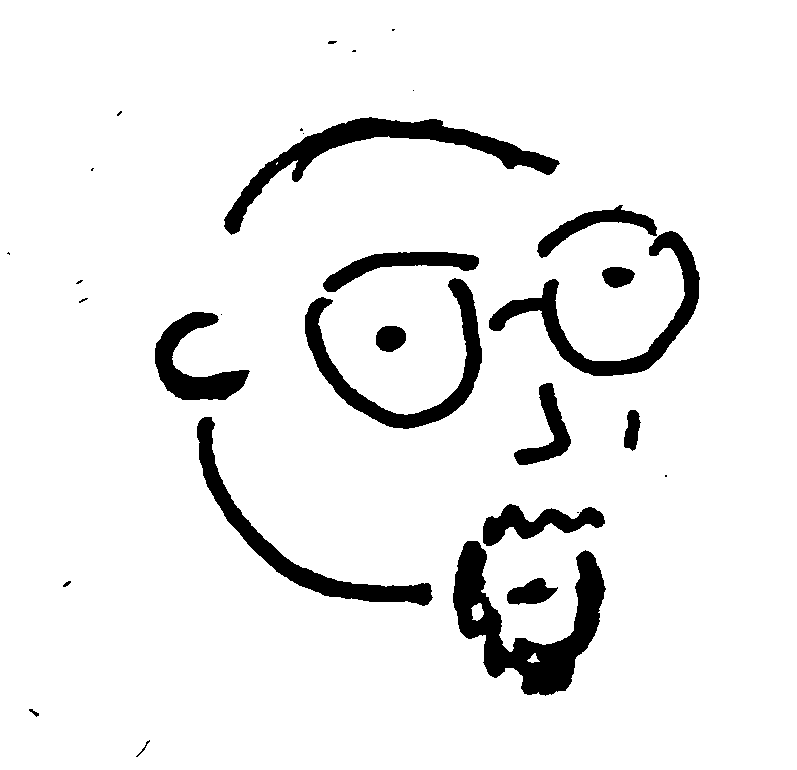
\includegraphics[width=5cm]{img-tombino/io_sx}};
			\node (example-textwidth-2) [right, align=left, text width=22cm, color=black, font=\fontsize{21pt}{22pt}\selectfont] at (6,0) {Come ricorda lo stesso Brownlee, il passo successivo fu esaminare i fotogrammi della telecamera posta in superficie:};
		\end{scope}
		%
		\begin{scope}[shift={(0,-136)}]
			\node at (21,0) {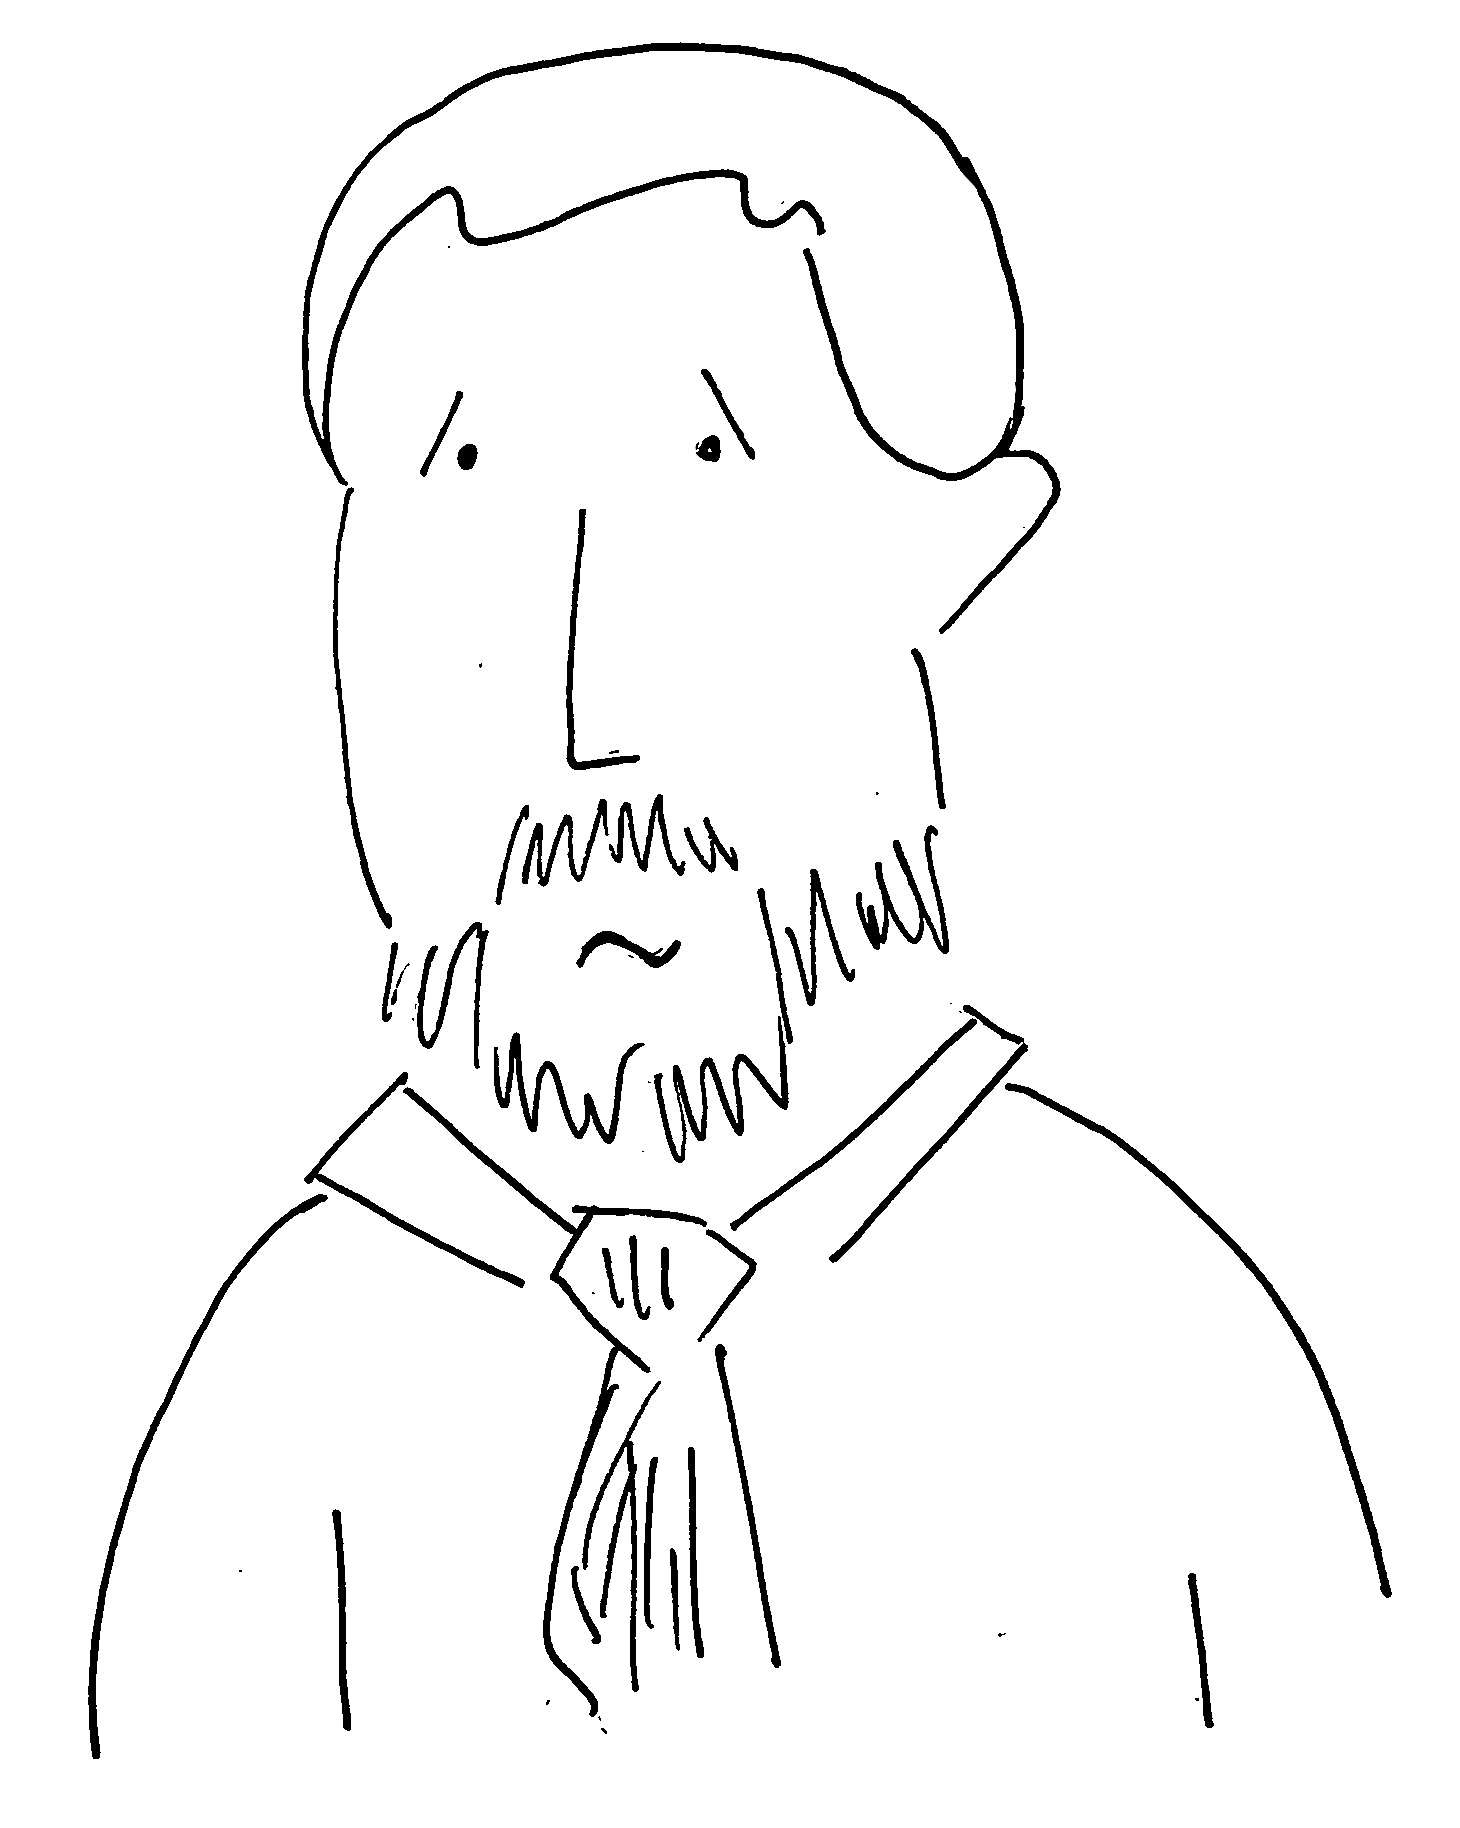
\includegraphics[width=8cm]{img-tombino/robert_brownlee}};
			\node (example-textwidth-2) [notice={(1,-0.5)}, ultra thick, right, align=center, text width=10cm, color=black, fill=white, font=\fontsize{23pt}{24pt}\selectfont] at (3,0) {Non ricordo quale fosse l'intervallo di tempo tra i fotogrammi, ma quando finii il mio esame, conclusi che il tombino andava veloce quanto un pipistrello.};
		\end{scope}
		%
		\begin{scope}[shift={(0,-145)}]
			\draw[color=black,fill=white,ultra thick] (1,2) rectangle (29,-2);
			\node at (3,0) {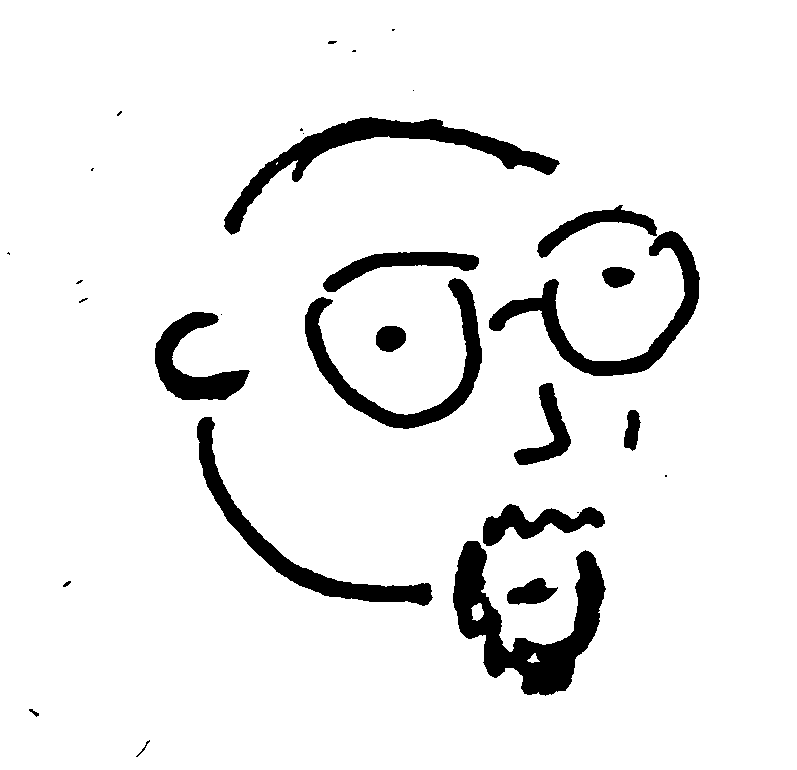
\includegraphics[width=5cm]{img-tombino/io_sx}};
			\node (example-textwidth-2) [right, align=left, text width=22cm, color=black, font=\fontsize{21pt}{22pt}\selectfont] at (6,0) {Nonostante queste conclusioni, fu probabilmente l'affermazione a denti stretti detta a Ogle che genero' la leggenda del tombino nello spazio!};
		\end{scope}
		%
		\begin{scope}[shift={(0,-150)}]
			\node at (27,0) () {
\includegraphics[width=3.7cm]{licenza}};
			\node at (18,-0.1) {\textcolor{black}{\fontsize{14}{15}\selectfont Testo e illustrazioni: @ulaulaman - Gianluigi Filippelli}};
		\end{scope}
	\end{tikzpicture}
%
\end{document}
